\section{Background Expectation}
The previous section described the set up of the X-ray Follow-Up including the 
expectation of generating quite a few alerts based on background events. It is 
crucial to understand the amount of the false positives to distinguish a 
possible signal contribution to the alert rate. An average background 
estimation is obtained by scrambling the neutrino singlets on the level of the 
Optical Follow-Up Filter.

The neutrino singlets on the level of the Optical Follow-Up Filter consist of 
about 80 - 90\% 
% (???) 
of atmospheric neutrinos and 10 - 20\% of 
misreconstructed muons. If a signal is present it will be suppressed  in 
comparison to the background. 
In the scrambling process the time and reconstruction information are split. 
While the time structure of the events is being kept in tact, incorporating 
possible time dependent rate changes, e.g. due to seasonal variations, for each 
scrambled result, the reconstruction information such as direction and quality 
is stripped of and randomly attributed to a different event time. An 
illustration is shown in Figure \ref{fig:scrambling_illustration}.
\begin{figure}[h]
 \centering
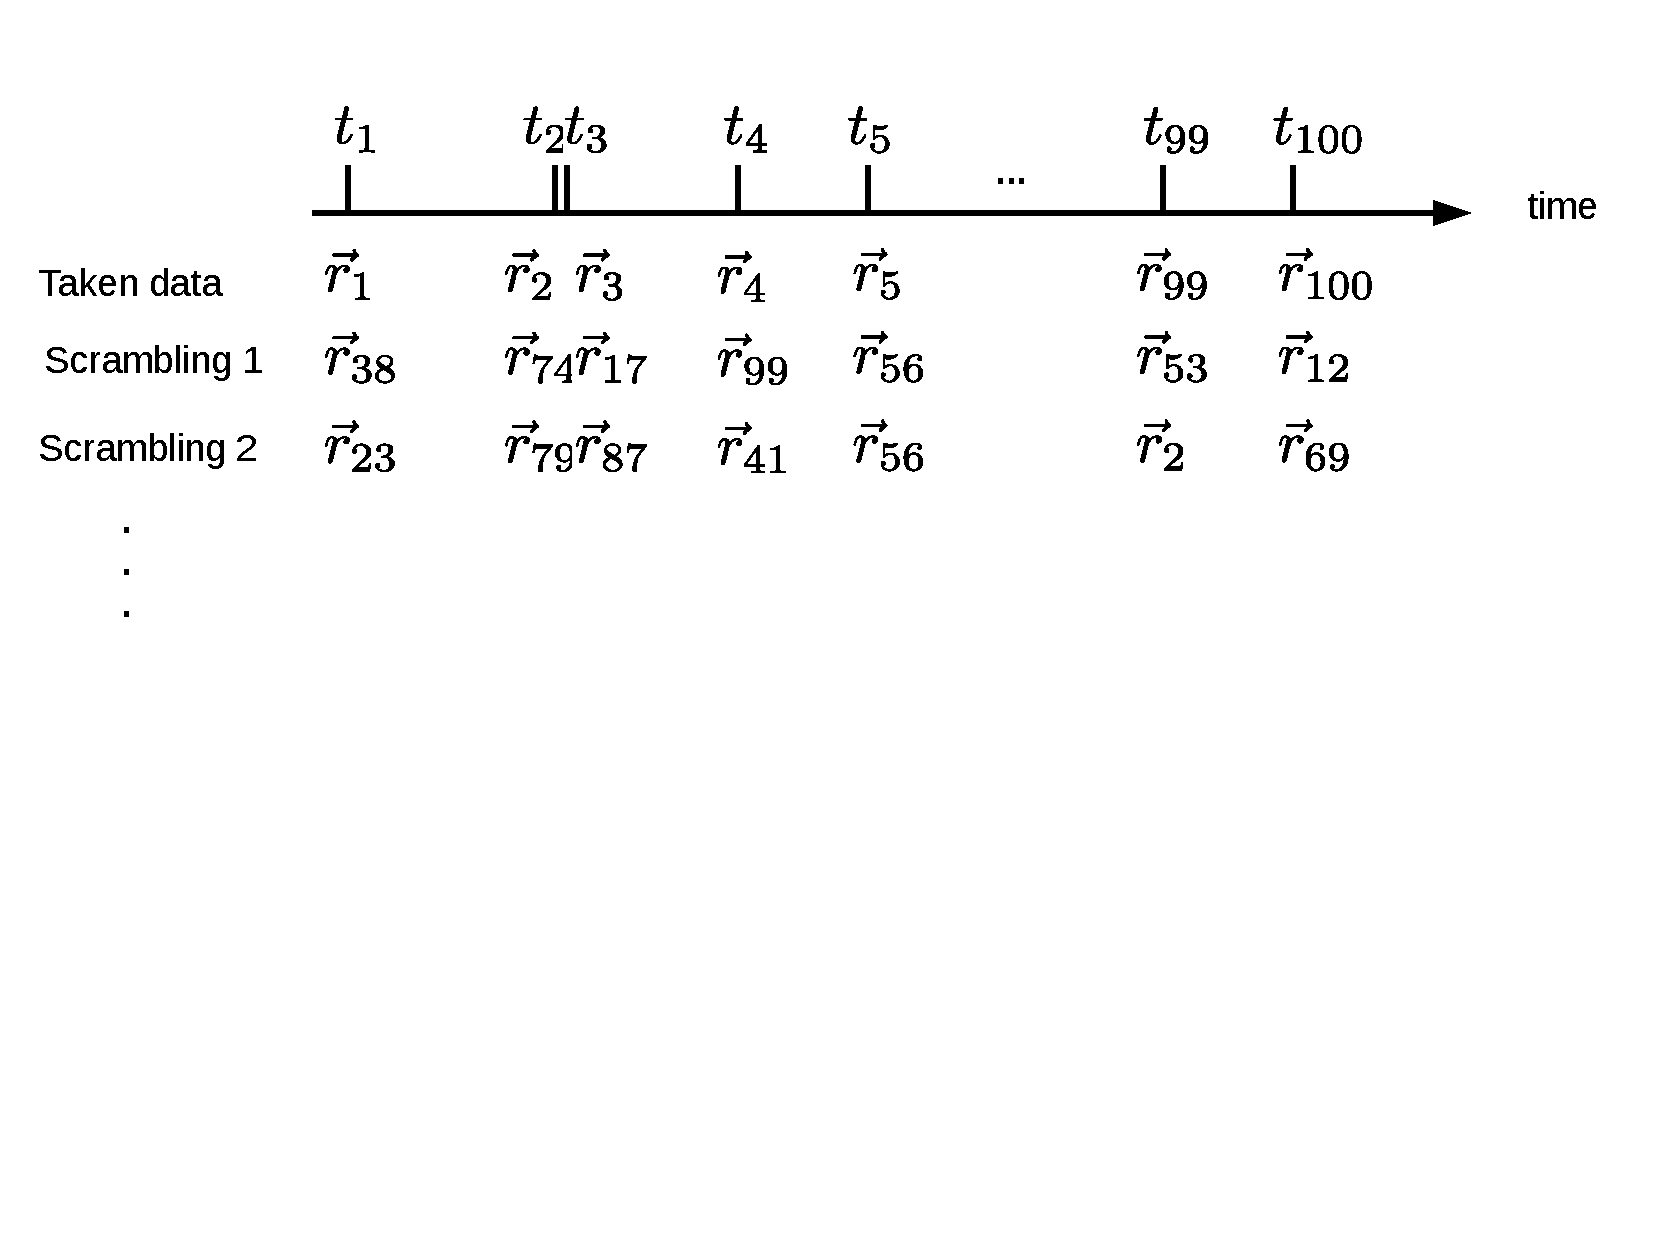
\includegraphics[trim=0cm 10.5cm 1cm 
1cm,clip=true,width=0.65\textwidth]{fig/scrambling_illustration.pdf}
\caption{An illustration of the scrambling process for an example of 100 
events. The time structure stays the same while the directional information is 
appointed to a new time randomly with each scrambling.}
\label{fig:scrambling_illustration}
\end{figure}

Events considered in the background estimation should only be events that 
actually were able to contribute to the triggered alerts, i.e. events detected 
while the Follow-Up system was operational. Towards that end all OFU singlets 
were extracted from the database and a time filter 
developed to exclude events happening during the Follow-Up downtime.
There can be several reasons that have to be included in the filter. Only data 
taken during good physics runs are considered. The good-run decision is based 
on a goodrun list extracted from i3live. The snapshot numbers are listed in 
 Table \ref{tab:goodrunlists}.

\begin{table}[h]
  \centering
  \begin{tabular}{l||c|c|c}
  Season & IC86-1 & IC86-2 & IC86-3 \\
  \hline
  snapshot & 94 & 109 & 93 \\
  \end{tabular}
  \caption{The snapshot numbers of the goodrun lists used for the different 
seasons.}
  \label{tab:goodrunlists}
\end{table}
Any real alert that was triggered during the three years considered in this 
analysis that occurred during a bad run is excluded in this analysis.

However, the good run list only evaluates the normal function of the IceCube 
detector but does not include downtime that is isolated to the Follow-Up 
System. Reasons can be various from software problems only affecting the OFU 
system to transmission problems via the ITS satellite.

\begin{table}[h]
  \centering
  \begin{tabular}{l|c|c|c}
   Season & IC86-1 & IC86-2 & IC86-BDT \\
\hline
   livetime [d] & 233.56 & 235.42 & 407.38 \\
   uptime [\%] & 0.91 & 0.90 & 0.89 \\
\hline
   expected Swift & 5.42 & 6.49 & 5.7 \\
   measured Swift & 6 & 5 &  7 \\
\hline
   expected multiplets & 0.044 & 0.063 &  0.073 \\
   measured multiplets & 0 & 0 & 0 \\
  \end{tabular}
  \caption{The table lists both the uptime of the Optical Follow-Up system and 
the results of the data scrambling to estimate the average background rate. The 
measured values are documented here for comparison.%rms values?
}
  \label{tab:scrambling_results}
\end{table}
The OFU uptime is 
evaluated using the test alerts that are designed to monitor the OFU systems.
On average, a test alert is expected to arrive every ten minutes. For this 
analysis, the system is considered 'down' if there is no test alert in a 
window twenty minutes after a test alert and twenty minutes before the next 
alert. This procedure averages over the effects that the system might crash 
directly after a test alert or that a new test alert arrives directly after the 
restart of the system and that the system is running though no test alerts 
arrived for over twenty minutes.

Using this time mask, all online alerts could be reproduced by re-analyzing the 
data offline and no new alerts were found. On average, 5.4, 6.5 and 5.7 Swift 
doublets were expected during the different seasons while the higher multiplet 
rate expectation varies between 0.044 and 0.073 (Table 
\ref{tab:scrambling_results}). An example of the scrambled distributions of 
expected Swift alerts during the IC86-1 season can be seen in Figures
\ref{fig:swift_scrambling} and \ref{fig:swift_scrambling_cum}.

The OFU system had an average uptime of 90\%. 
This includes downtime for OFU unrelated reasons like calibration runs.

\begin{figure}[h]
\centering
 \captionsetup{width=.9\textwidth}
%  \captionsetup{margin=0pt}
\subfloat[The differential distribution \label{fig:swift_scrambling}]{%
 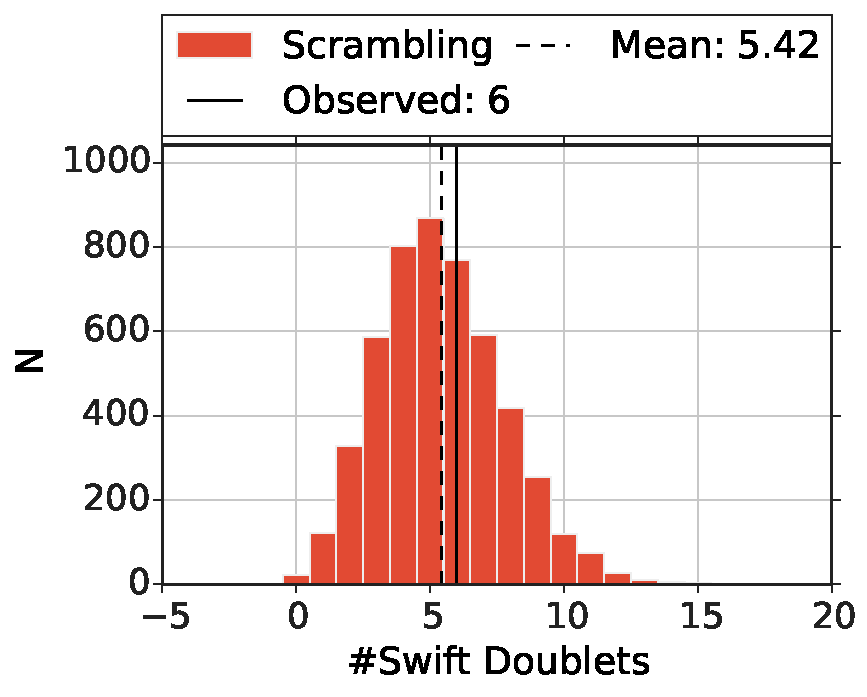
\includegraphics[width=0.45\textwidth]{fig/swift_scrambling.pdf}}
 \subfloat[The inverse cumulative distribution.
\label{fig:swift_scrambling_cum}]{%
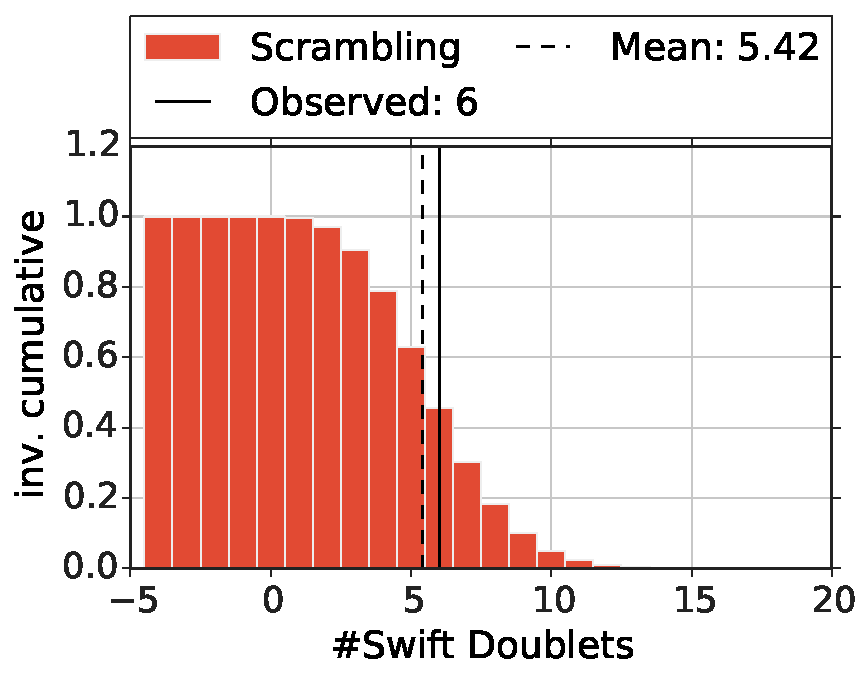
\includegraphics[width=0.45\textwidth]{fig/swift_scrambling_cum.pdf}}
\caption{The differential and inverse cumulative distributions of 
detectable Swift doublets for a hundred thousand scrambled datasets. The 
distributions for 
IC86-1 was chosen.}
\end{figure}



% error on livetime and mean value in an example? like decrease to 10 min? and 
% increase to 30 min?
% 
% table with uptime and mean values. quadruplets?
% 
% plots for three seasons? or is one season enough?
% 
% split the table up. part into Optical Follow-Up filter part into results. 
% though the p-values are not calculated according to the significance section. 
% livetime/uptime doesn't fit for IC86-1
% \begin{table}[h]
%   \centering
%   \begin{tabular}{l|c|c|c}
%    Season & IC86-1 & IC86-2 & IC86-BDT \\
% \hline
%    livetime [d] & 233.56 & 235.42 & 407.38 \\
%    uptime [\%] & 0.96 & 0.90 & 0.89 \\
% \hline
%    expected Swift & 5.42 & 6.49 & 5.7 \\
%    measured Swift & 6 & 5 &  7 \\
%    p value & 0.45 &  0.79 & 0.34 \\
% \hline
%    expected multiplets & 0.044 & 0.063 &  0.073 \\
%    measured multiplets & 0 & 0 & 0 \\
%    p value & 1 & 1 & 1\\
%   \end{tabular}
%   \caption{}
%   \label{tab:scrambling_results}
% \end{table}